\documentclass[a4paper, 12pt, french]{article}
\usepackage[utf8]{inputenc}
\usepackage[T1]{fontenc}
\usepackage{babel}
\usepackage{setspace}
\usepackage{hyperref}
\usepackage{imakeidx}
\usepackage{graphicx}
\usepackage{fancyhdr}
\usepackage{chngcntr}
\usepackage{pifont}
\usepackage{xcolor}
\usepackage{glossaries}
\usepackage{helvet}
\usepackage{titlesec}
\usepackage{tikz}
\usepackage{rotating}
\usepackage{lscape}
\usepackage{wrapfig}
\usepackage[stable]{footmisc}

\makeindex[intoc]
 
\counterwithin{figure}{section}
\counterwithin{table}{section}

\definecolor{ssiYellow}{RGB}{255,237,0}
\definecolor{ssiRed}{RGB}{231,0,14}
\definecolor{ssiBlack}{RGB}{18,18,13}

\newcommand{\bdot}{\item[\color{ssiYellow}\ding{108}]} 
\newcommand{\bdotoutlined}{\item[\color{ssiYellow}\ding{109}]}
\newcommand{\bsquare}{\item[\color{ssiYellow}\ding{110}]} 

\hypersetup{pdfborder = {0 0 0}}
\renewcommand{\familydefault}{\sfdefault}

\titleformat{name=\section}{\normalfont\Large\bfseries\color{ssiBlack}}{\color{ssiYellow}\rule[-1.35mm]{3em}{1.25em}{\color{white}\hspace{-1cm}\normalfont\Large\bfseries\thesection\hspace{15pt}}}{1em}{}[\color{ssiYellow}{\titlerule[4pt]}\vspace*{4pt}]
\titleformat{\subsection}{\normalfont\Large\bfseries\color{ssiBlack}}{\color{ssiRed}\rule[-1.35mm]{3em}{1.25em}{\color{white}\hspace{-1.3cm}\normalfont\Large\bfseries\thesubsection\hspace{10pt}}}{1em}{}[\color{ssiYellow}{\titlerule[3pt]}\vspace*{4pt}]
\titleformat{\subsubsection}{\normalfont\Large\bfseries\color{ssiBlack}}{\color{ssiYellow}\rule[-1.35mm]{3em}{1.25em}{\color{white}\hspace{-1.60cm}\normalfont\Large\bfseries\thesubsubsection\hspace{5pt}}}{1em}{}[\color{ssiYellow}{\titlerule[2pt]}\vspace*{4pt}]

\titleformat{name=\section,numberless=true}{\color{ssiBlack}\normalfont\Large\bfseries}{}{0em}{}[\color{ssiYellow}{\titlerule[4pt]}\vspace*{4pt}]
\titleformat{name=\subsection,numberless=true}{\color{ssiBlack}\normalfont\Large\bfseries}{}{0em}{}[\color{ssiYellow}{\titlerule[3pt]}\vspace*{4pt}]
\titleformat{name=\subsubsection,numberless=true}{\color{ssiBlack}\normalfont\Large\bfseries}{}{0em}{}[\color{ssiYellow}{\titlerule[2pt]}\vspace*{4pt}]

\sloppy

\pagestyle{fancy}
\fancyhf{}
\rhead{Informatique et réseaux}
\lhead{PINEAU Anthony}

\begin{document}
	\begin{titlepage}
		\begin{center}

			\tikz[remember picture,overlay] \node[opacity=0.3,inner sep=0pt] at (current page.center){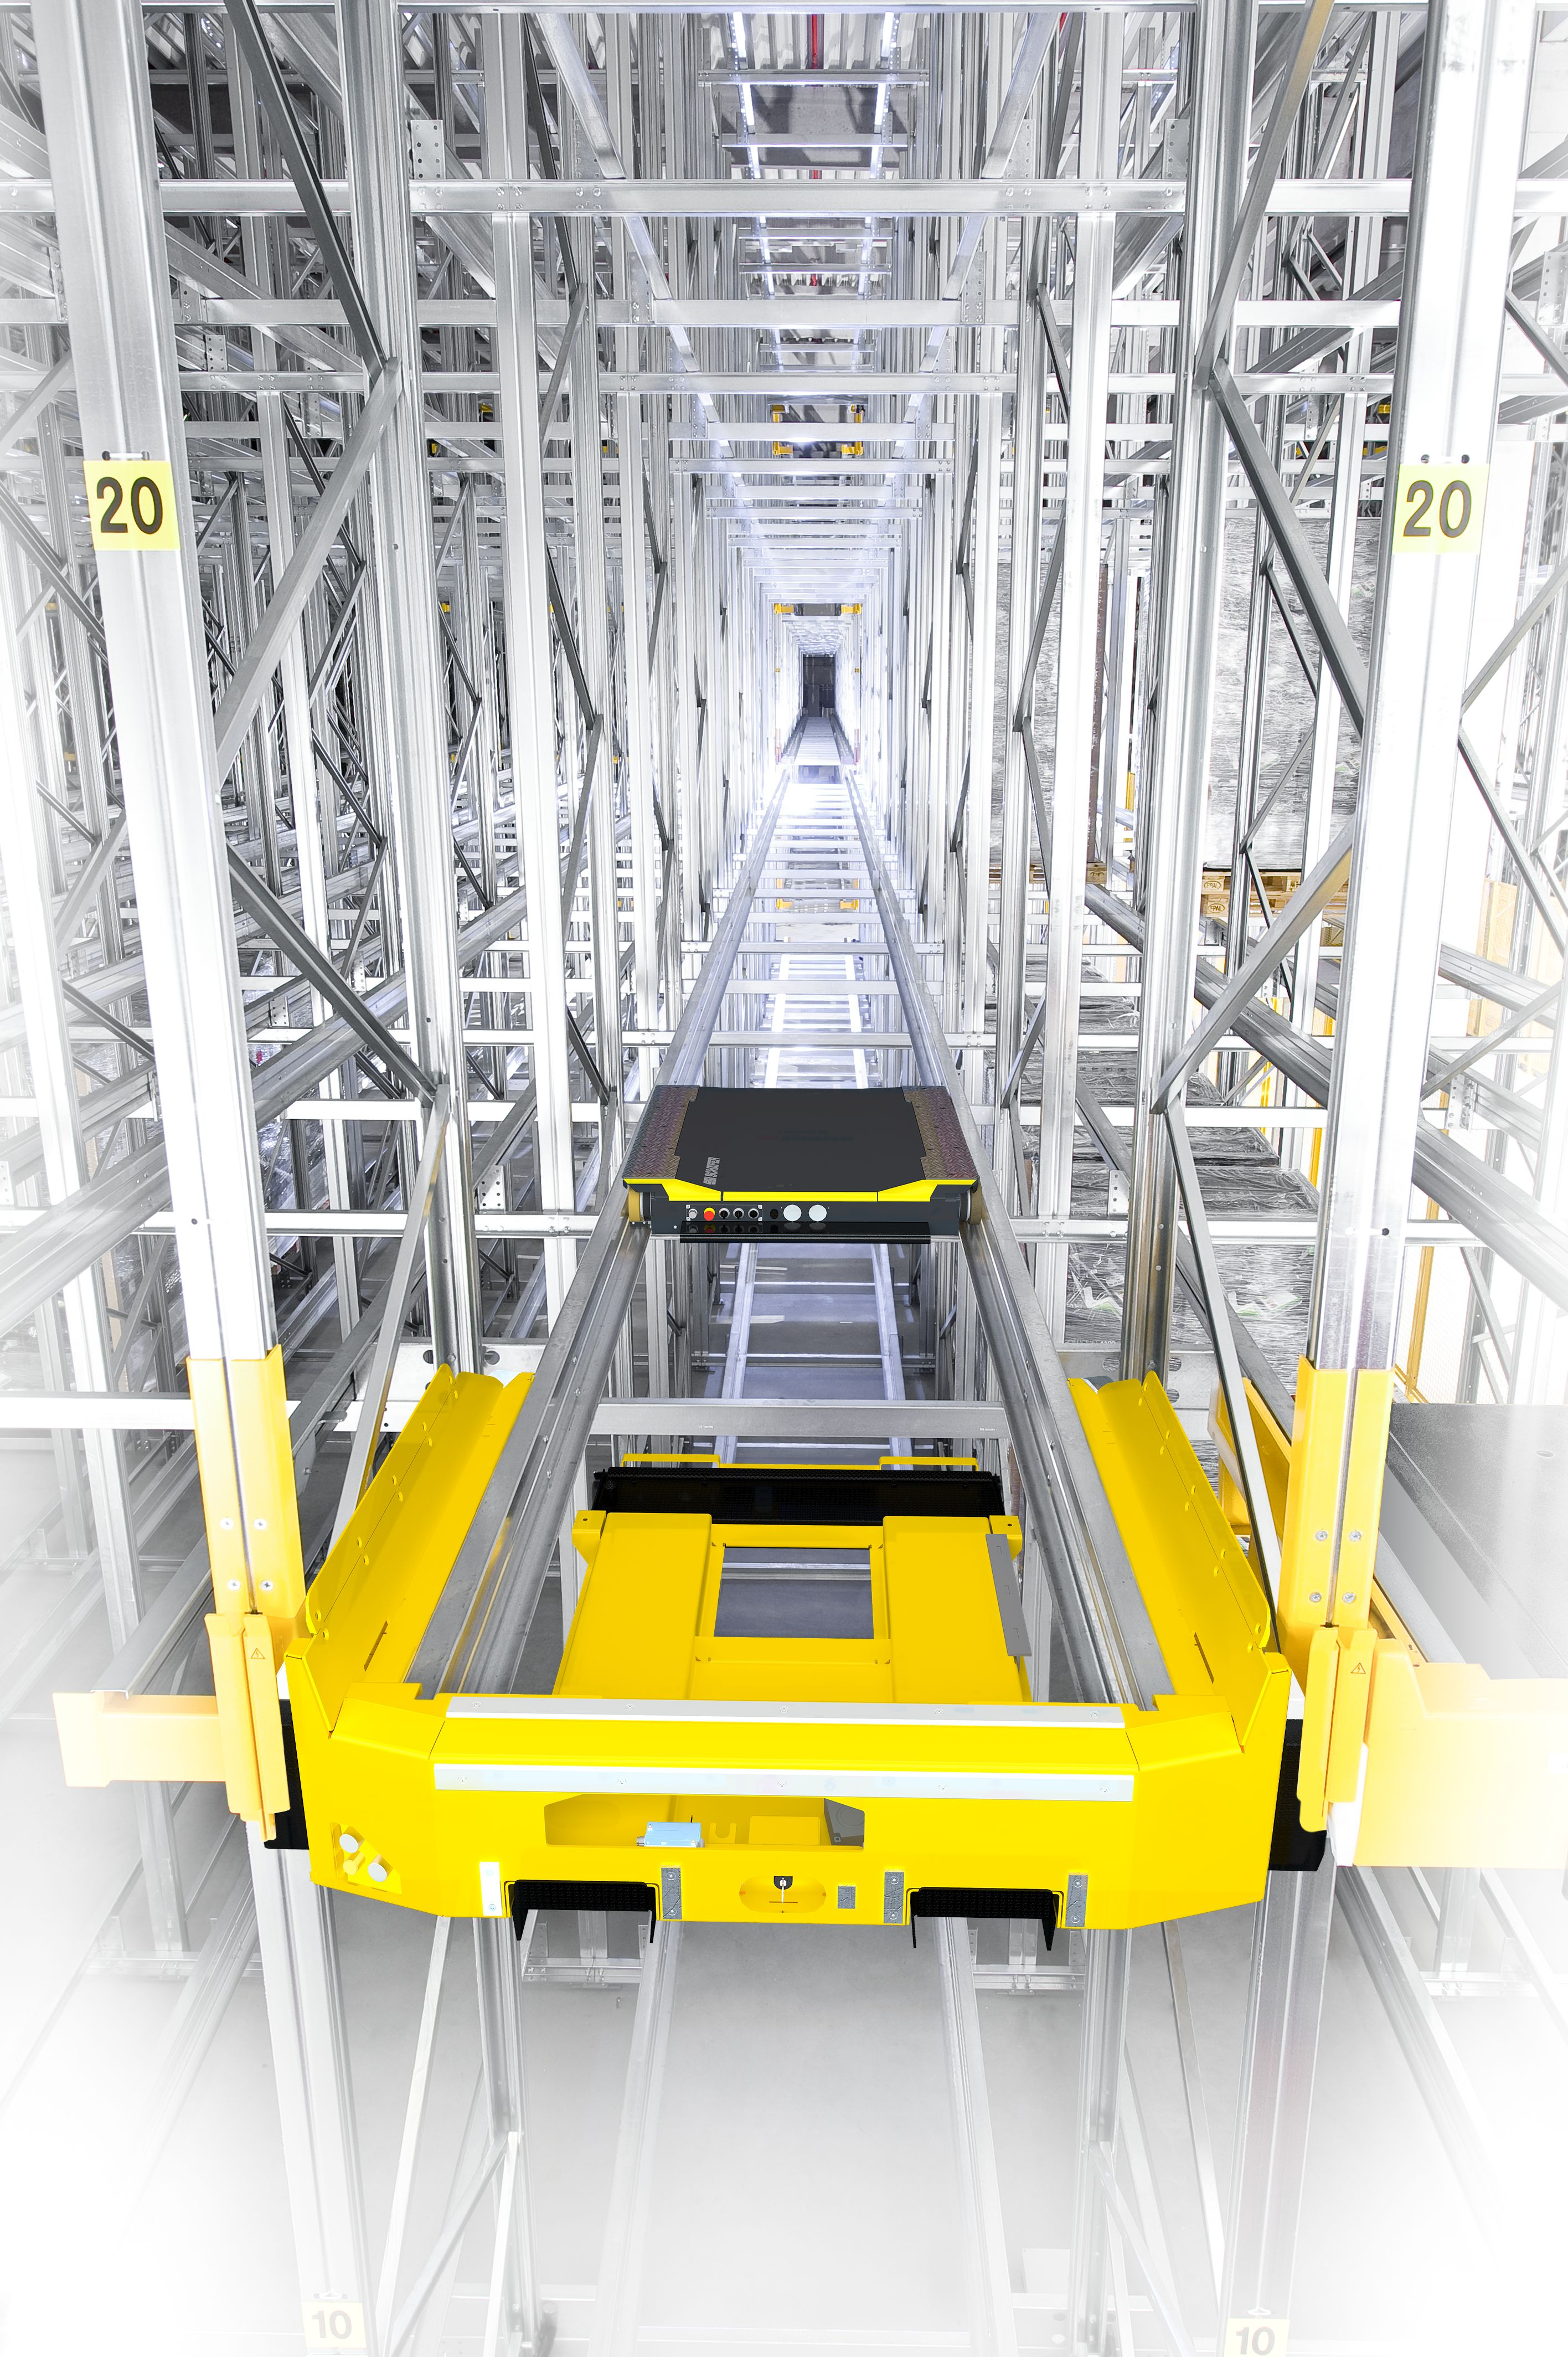
\includegraphics[width=\paperwidth,height=\paperheight]{../memoire/images/ssi_orbiter_highlight.jpg}};

			%\vspace*{1cm}

			\Huge
			\textbf{Rapport d'avancement}

			\vspace{0.5cm}
			\LARGE
			"Passer d'une application client lourd à une application web"

			\vspace{1.5cm}

			\textbf{Anthony PINEAU}\\
			\textbf{IR2023}

			\vfill

			
\includegraphics[width=0.6\textwidth]{../memoire/images/schaefer.jpg}
			\vfill
			
\includegraphics[width=0.4\textwidth]{../memoire/images/esaip.jpg}

			\vfill

			Période effectuée du\\
			28 août 2023 au 22 septembre 2023

			\vspace{0.8cm}
			
			\Large
			Maître de stage : Monsieur Thierry NEROT\\
			Tuteur pédagogique : Docteur Sofiane HAMRIOUI\\
		\end{center}
	\end{titlepage}
		
	\newpage
	
	\doublespacing
	\tableofcontents
	
	\phantomsection
	\listoffigures
	\addcontentsline{toc}{section}{\listfigurename}
	
	\newpage
		
	\rfoot{Page \thepage}
	
	\singlespacing

	\section{Objectifs de la période et mise en évidence de tout changement stratégique}
		Les objectifs de cette période ont été de continuer à développer l'application web en reactjs, ainsi que de rédiger la documentation du projet. J'ai aussi pu travailler sur la rédacton de mon mémoire pendant le stage. Il n'y a pas eu de changement stratégique particulier.

	\section{Travaux réalisés}
		Voici la liste des travaux réalisés au cours de cette période :
		\begin{itemize}
			\bdot{Développement de l'application web}
			\bdot{Rédaction documentation}
			\bdot{Rédaction mémoire}
		\end{itemize}		

	\section{Difficultés rencontrées}
		Aucune difficulté particulière rencontrée durant cette période.

	\newpage
	
	\section{Suite des travaux}
		\begin{figure}[h!]
			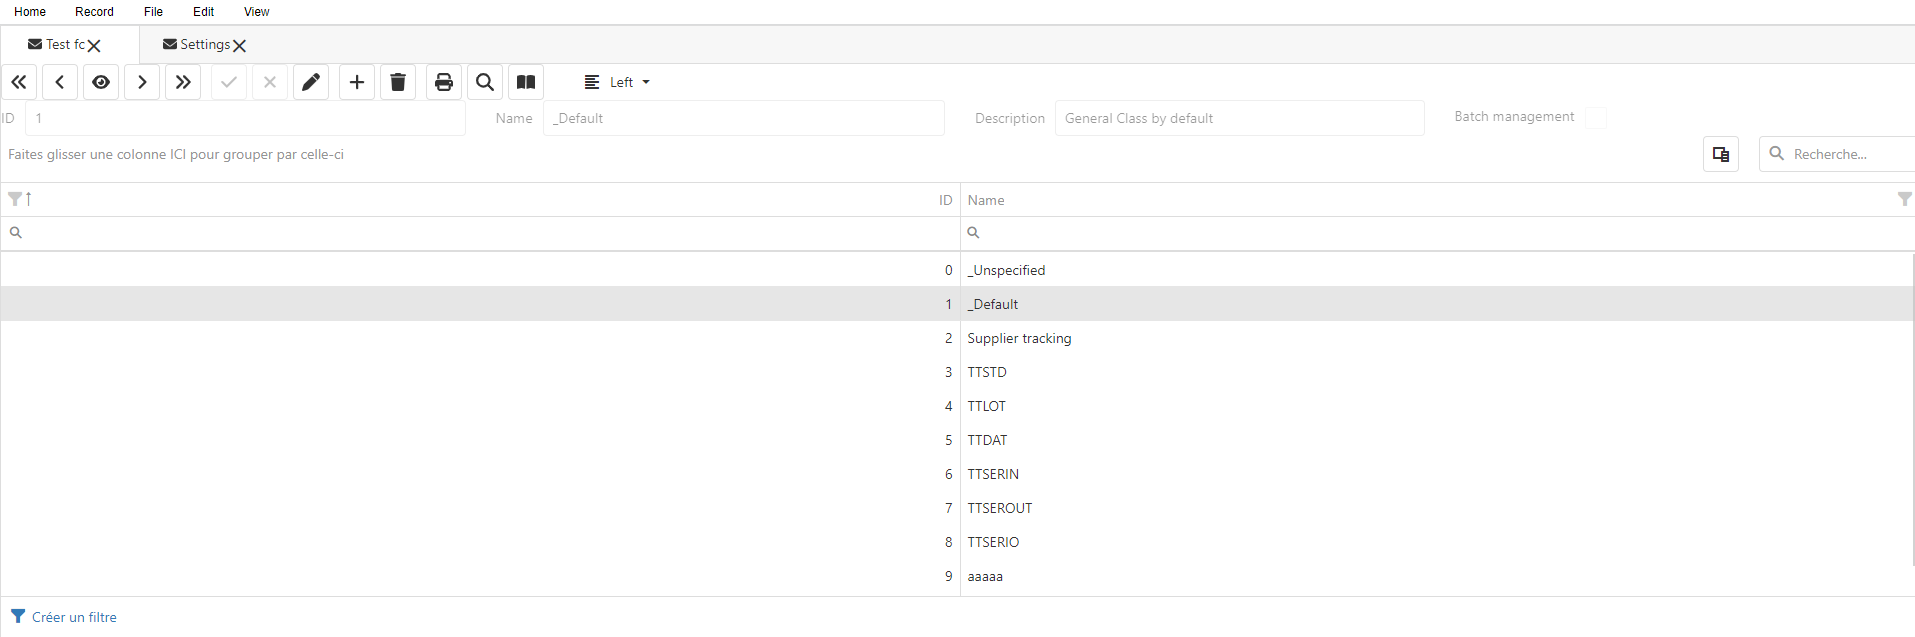
\includegraphics[width=\linewidth]{mph_web_reactts_aout_1.png}
			\caption{Capture d'écran de l'application développée avec ReactJS}
		\end{figure}
		\begin{figure}[h!]
			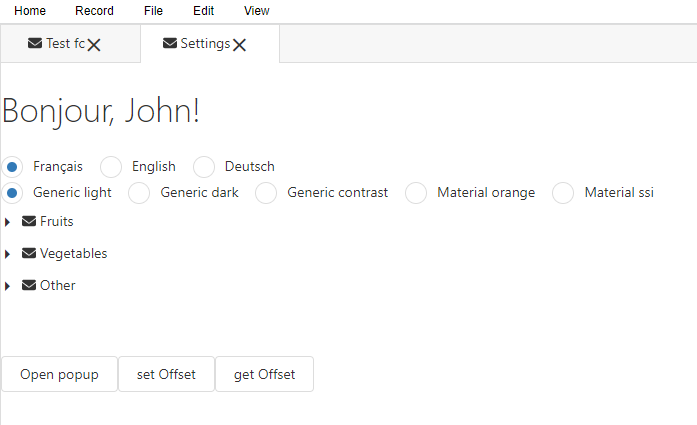
\includegraphics[width=\linewidth]{mph_web_reactts_aout_2.png}
			\caption{Capture d'écran de l'application développée avec ReactJS}
		\end{figure}
		
		\newpage
		
		\begin{figure}[h!]
			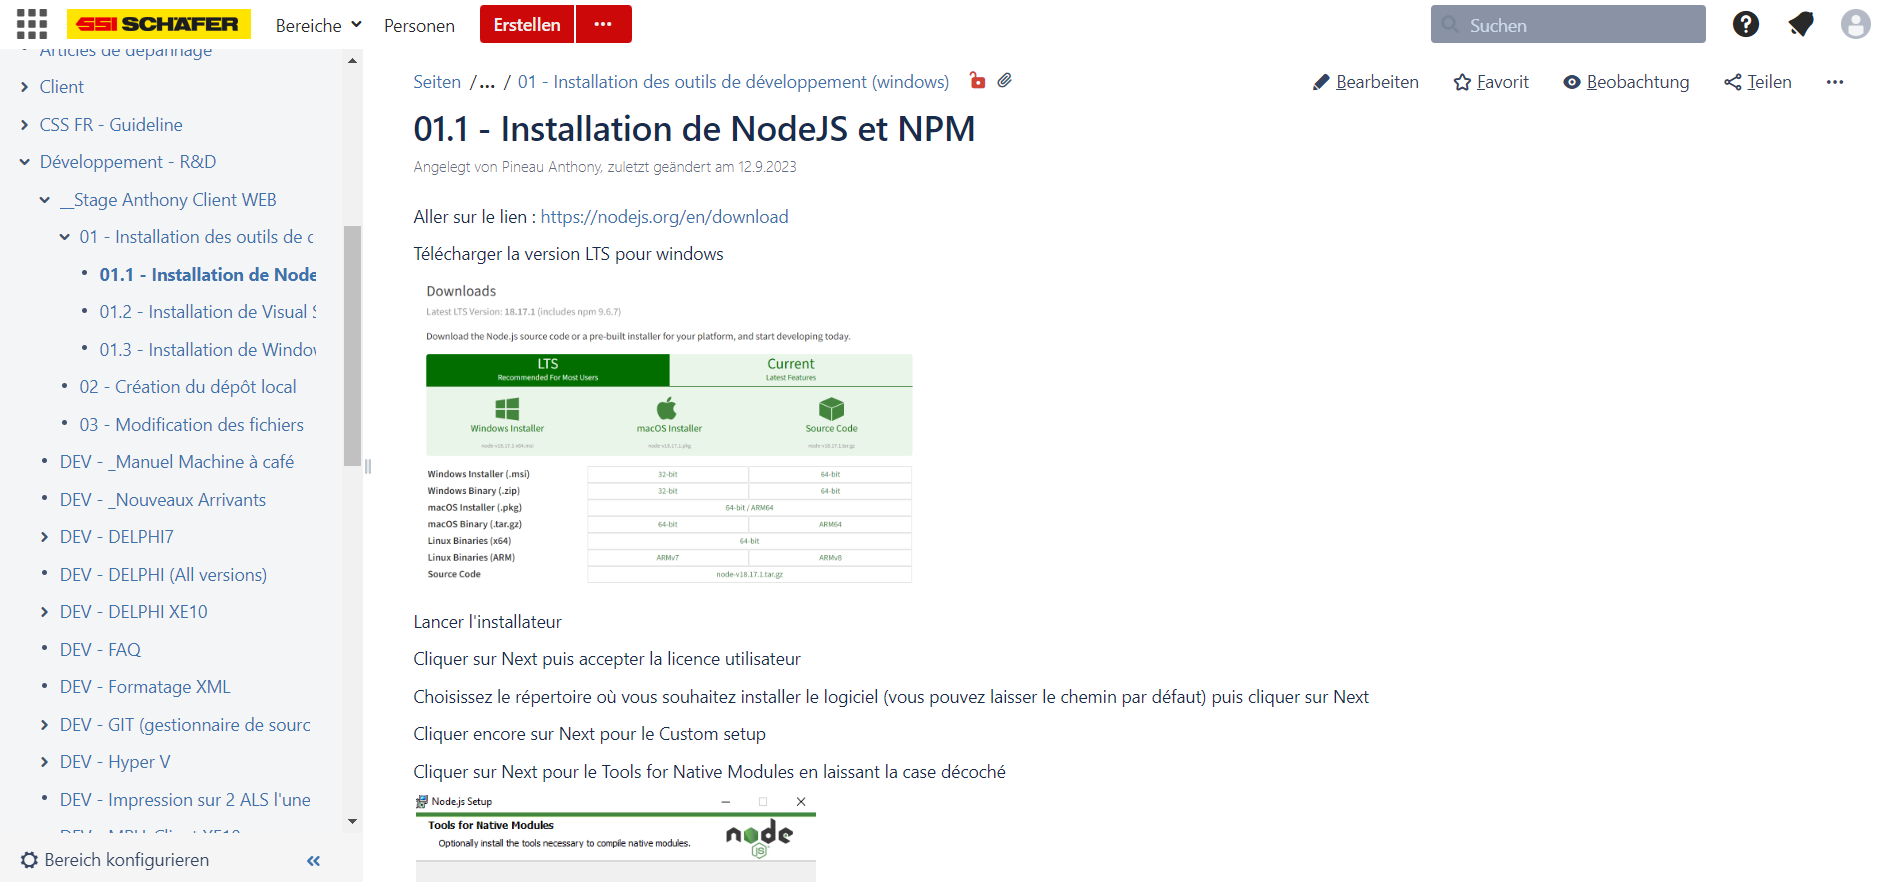
\includegraphics[width=\linewidth]{confluence_nodejs.png}
			\caption{Capture d'écran de la documentation produite sur confluence}
		\end{figure}
		\begin{figure}[h!]
			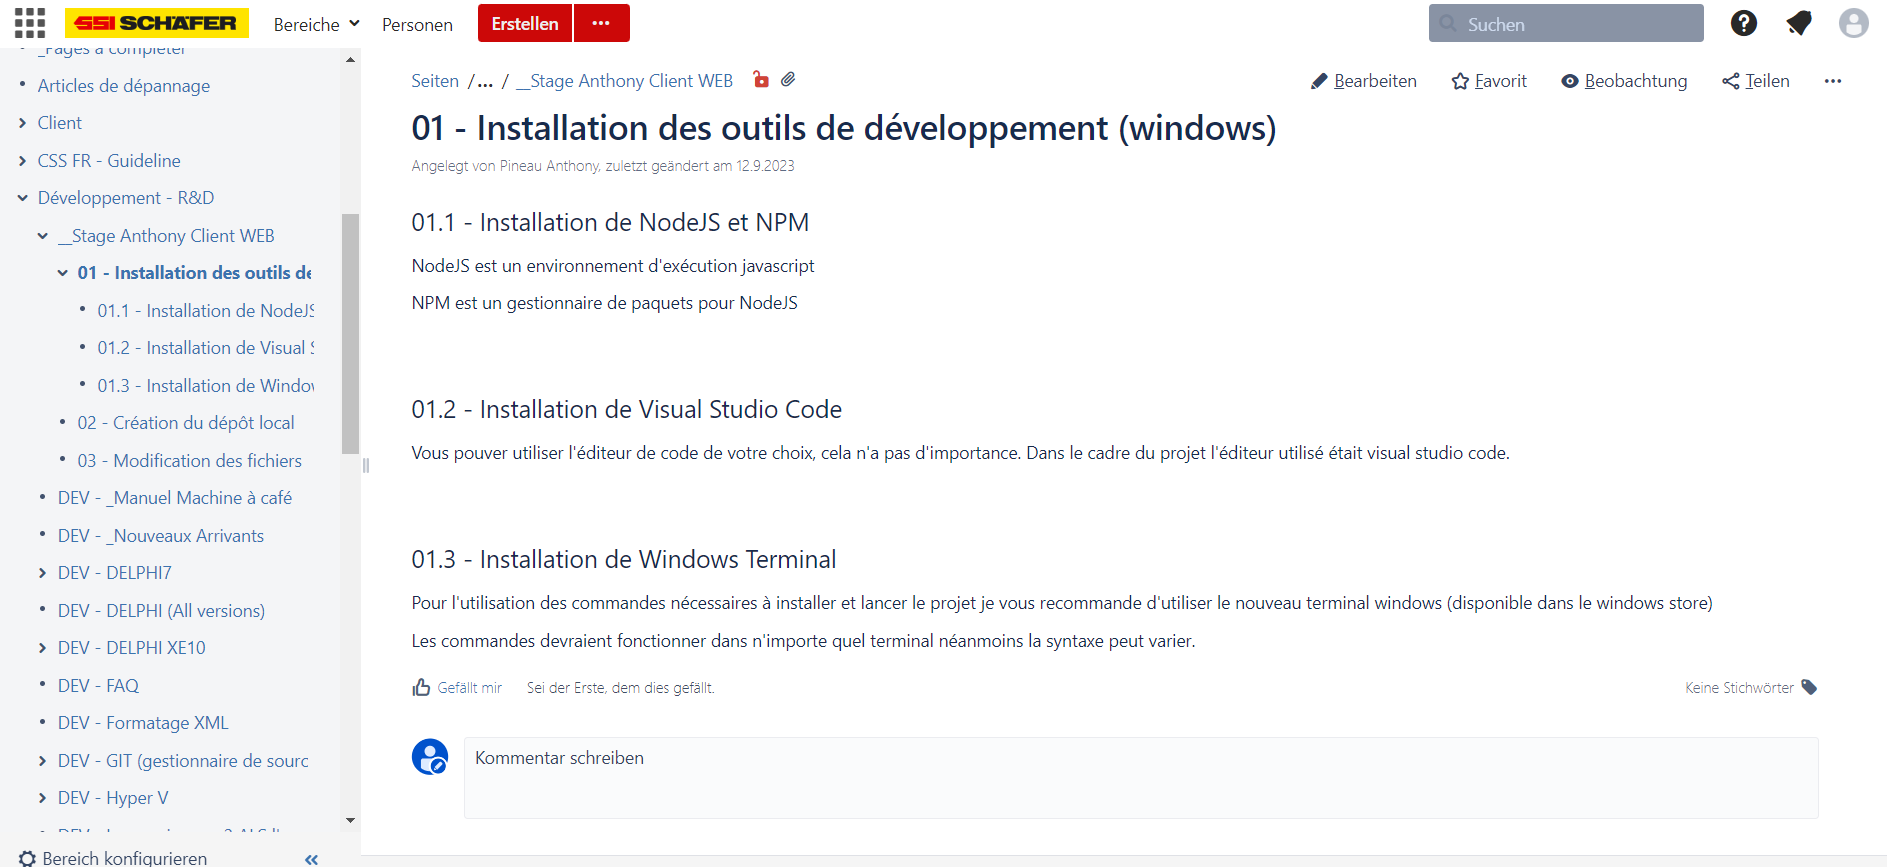
\includegraphics[width=\linewidth]{confluence_tools.png}
			\caption{Autre capture d'écran de la documentation produite sur confluence}
		\end{figure}
		
	\newpage

	\section{Mise à jour du planning du projet}
		\begin{figure}[h!]
			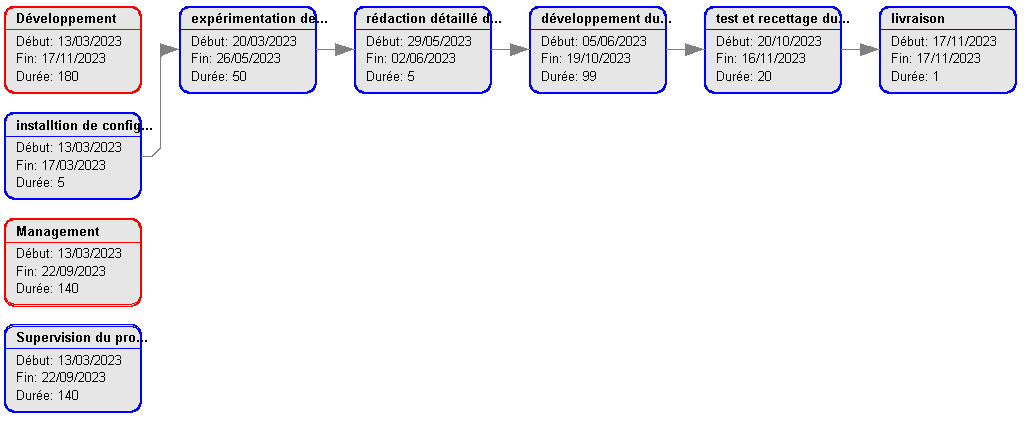
\includegraphics[width=\linewidth]{gantt_13_04_13_05.png}
			\caption{Diagramme de PERT du diagramme de GANTT inchangé durant la période du 28/08 au 22/09}
		\end{figure}
		
		
\end{document}